% =====================================================================
% 03b_infrastructure_adhoc.tex
% Mo hinh Infrastructure va Ad-hoc (IBSS): doi chieu chi tiet + so do thuc te.
% Nguon: "Mo hinh infrastructure.docx", bo anh "picture source" (Picture1-6)
% va 3 so do "picture source/so do" (N09_sodo1_infrastructure,
% N09_sodo2_adhoc, N09_sodo3_thanhphan).
% Duoc \input ngay sau sections/03_architecture.tex nen cac tieu de duoi day
% tiep tuc danh so trong cung Muc "Kien truc va cac thanh phan WLAN".
% =====================================================================
\begingroup
\newcolumntype{L}[1]{>{\hsize=#1\hsize\raggedright\arraybackslash}X}

\subsection{Mô hình hạ tầng (Infrastructure) và mô hình tùy biến (Ad-hoc)}

Trong phạm vi gia đình và doanh nghiệp nhỏ, mạng cục bộ không dây thường được
thiết lập theo hai mô hình chính: mô hình hạ tầng (Infrastructure, có thiết bị
trung tâm) và mô hình tùy biến hay ngang hàng (Ad-hoc). Mô hình hạ tầng là lựa
chọn phổ biến gần như mặc định, trong khi mô hình Ad-hoc trên các thiết bị đầu
cuối thông dụng đã dần được thay thế bởi các công nghệ ngang hàng mới hơn như
Wi-Fi Direct, và chỉ còn tồn tại bền vững trong những dạng tiến hóa chuyên biệt
(MANET, VANET, FANET) ở các lĩnh vực không có hạ tầng cố định.

\subsubsection{Mô hình hạ tầng (Infrastructure)}

Đây là một hệ thống phân cấp: một nhóm thiết bị đóng vai trò quản lý và cung cấp
dịch vụ, nhóm còn lại đóng vai trò thụ hưởng. Ba thành phần thiết bị chính gồm:

\begin{itemize}[leftmargin=*]
  \item \textbf{\acf{ap} / bộ định tuyến không dây:} phát sóng Wi-Fi (công bố
    \ac{ssid}), nhận và chuyển tiếp dữ liệu giữa các thiết bị không dây với nhau
    và giữa thiết bị không dây với mạng Internet nếu có. Trong hộ gia đình, thiết
    bị này thường tích hợp thêm chức năng modem (giải điều chế tín hiệu của nhà
    cung cấp dịch vụ) và switch (chia cổng mạng có dây).
  \item \textbf{Thiết bị đầu cuối (\acp{sta}):} mọi thiết bị có card mạng không
    dây (WNIC -- Wireless Network Interface Card) như máy tính xách tay, điện
    thoại thông minh, Smart TV, camera Wi-Fi hay bóng đèn thông minh; các trạm
    này chỉ sử dụng dịch vụ do \ac{ap} cung cấp.
  \item \textbf{Hạ tầng dây dẫn:} cáp mạng RJ45 hoặc cáp quang nối bộ
    định tuyến ra bên ngoài, hoặc nối tới các switch khác trong tòa nhà; đây
    chính là \ac{ds} đã trình bày ở Mục~\ref{sec:arch}.
\end{itemize}

Hình~\ref{fig:sodo-thanhphan} sơ đồ hóa các thành phần này trong một mạng WLAN
gia đình điển hình: đường truyền quang từ nhà cung cấp dịch vụ vào modem quang
(ONT), qua cổng WAN của bộ định tuyến tích hợp, rồi từ cổng LAN tỏa ra các thiết
bị đầu cuối. Sơ đồ cũng cho thấy một \ac{ap} mở rộng có thể được nối thêm bằng
cáp Ethernet để mở rộng vùng phủ, biến nhiều \ac{bss} rời rạc thành một
\ac{ess} thống nhất.

\begin{figure}[htbp]
  \centering
  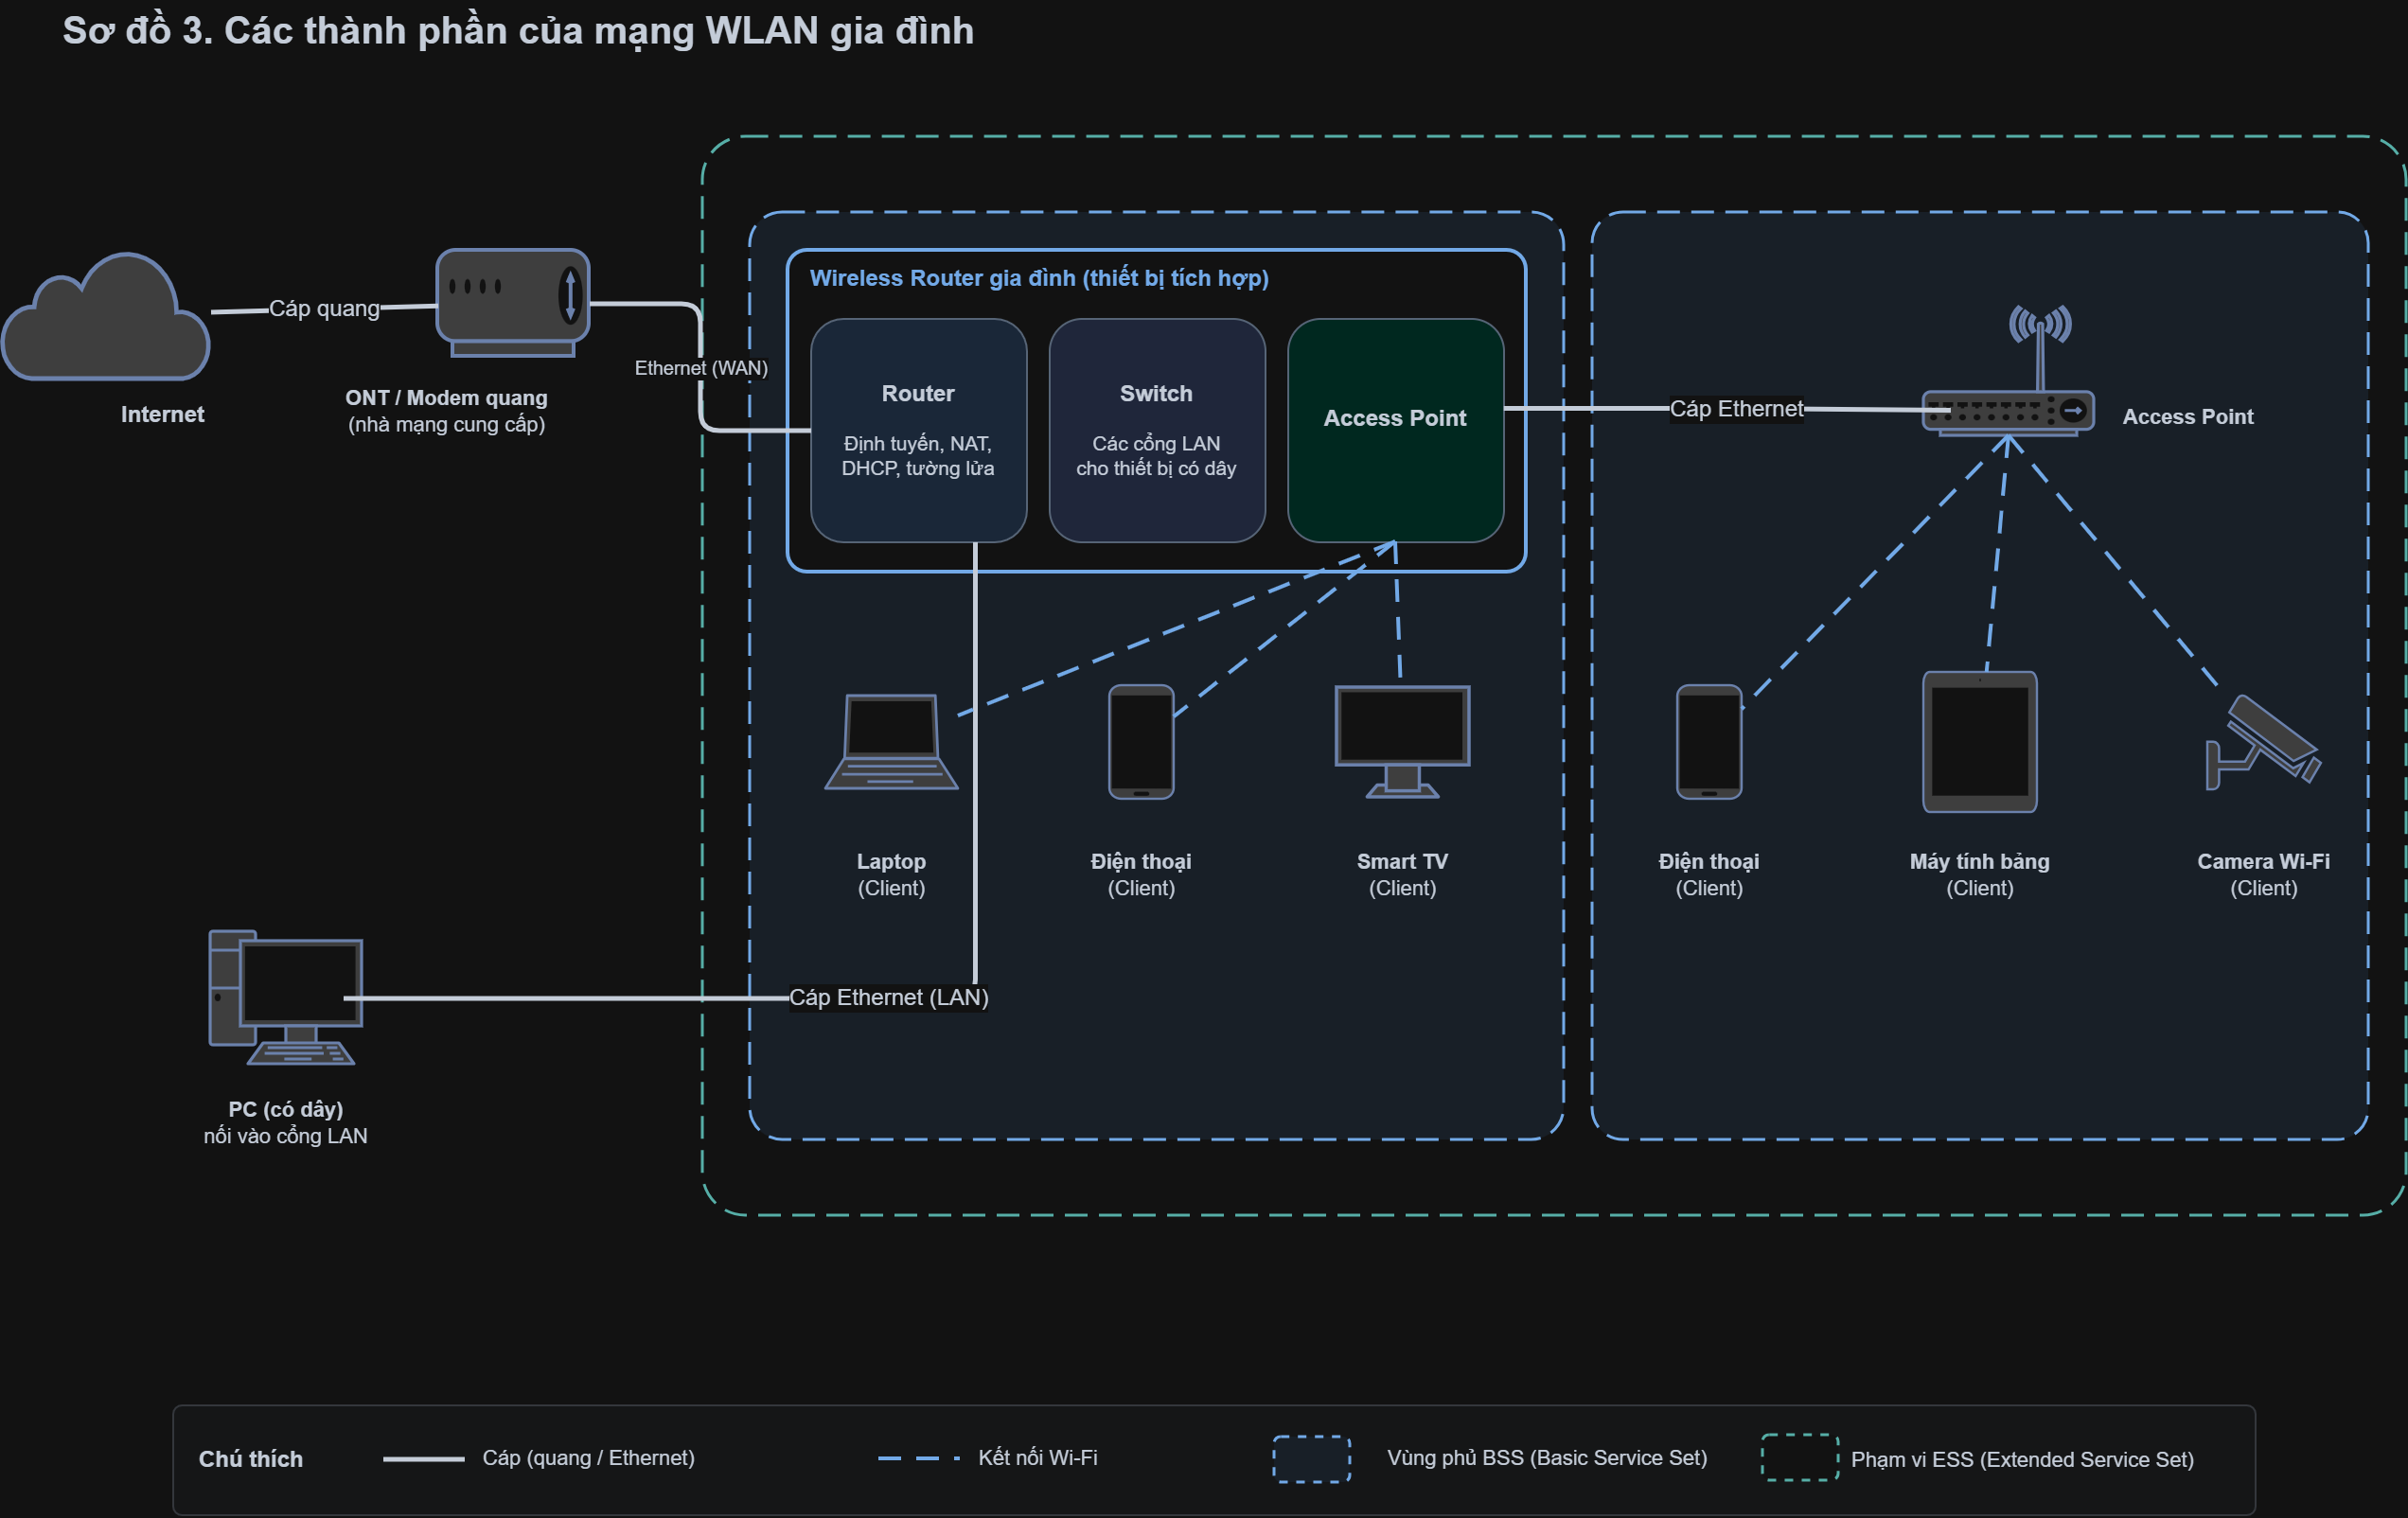
\includegraphics[width=\linewidth]{figures/N09_sodo3_thanhphan.png}
  \caption[Các thành phần của một mạng WLAN gia đình]{Các thành phần của một mạng WLAN gia đình: modem quang, bộ định tuyến
  tích hợp (định tuyến/NAT/DHCP, switch cổng LAN, \ac{ap}), các thiết bị đầu cuối
  không dây và thiết bị có dây; nét đứt thể hiện vùng phủ \ac{bss} và phạm vi
  \ac{ess}.}
  \label{fig:sodo-thanhphan}
\end{figure}

\textbf{Phạm vi định danh: \ac{bss} và \ac{bssid}.} \ac{bss} là đơn vị cấu
thành cơ bản nhất của mạng Wi-Fi theo mô hình hạ tầng: một \ac{ap} duy nhất cùng
toàn bộ thiết bị không dây đang liên kết trực tiếp với \ac{ap} đó. Để phân biệt
các \ac{bss} với nhau, mỗi \ac{bss} mang một mã định danh duy nhất là
\ac{bssid}, và trong mô hình hạ tầng \ac{bssid} chính là địa chỉ MAC vật lý của
giao diện vô tuyến trên \ac{ap}.

\textbf{Mở rộng và chuyển vùng: \ac{ess}.} \ac{ess} là mô hình mở rộng, hình
thành khi nhiều \ac{bss} (nhiều \ac{ap}) được nối với nhau qua \ac{ds} để phủ
sóng một không gian lớn hơn. Mọi \ac{ap} trong cùng một \ac{ess} dùng chung một
\ac{ssid} và cùng cấu hình bảo mật, mặc dù mỗi \ac{ap} vẫn sở hữu \ac{bssid}
riêng. Nhờ đó thiết bị đầu cuối có thể di chuyển liên tục giữa các vùng phủ sóng
mà không bị ngắt kết nối (roaming). Cần lưu ý rằng \ac{ess} truyền thống không
có cơ chế chuyển vùng nhanh, nên việc chọn \ac{ap} nào để liên kết là do chính
thiết bị của người dùng quyết định dựa trên cường độ tín hiệu; các tiêu chuẩn
802.11k/v/r sau này mới bổ sung cơ chế hỗ trợ chuyển vùng nhanh và cân bằng tải.

\subsubsection{Mô hình tùy biến (Ad-hoc / IBSS)}

Mô hình Ad-hoc là một mạng lưới phi tập trung: không có thiết bị nào làm chủ và
tất cả các nút đều bình đẳng. Thành phần thiết bị chỉ gồm các nút không dây
(\emph{wireless nodes}) -- chính là các thiết bị đầu cuối như máy tính xách tay
hay máy tính để bàn gắn card/USB Wi-Fi -- và không có điểm truy cập trung tâm.
Trong mạng nhiều chặng, các nút có thể được cấu hình thêm để chuyển tiếp gói tin
và thực hiện định tuyến; IBSS cơ bản chỉ cung cấp liên lạc trực tiếp giữa các
nút trong cùng vùng phủ sóng. Hình~\ref{fig:sodo-adhoc} mô tả dạng triển khai hai nút mà nhóm dùng để
kiểm chứng mô hình này (xem Mục~\ref{sec:adhoc-config} và
Mục~\ref{sec:experiment}).

\begin{figure}[htbp]
  \centering
  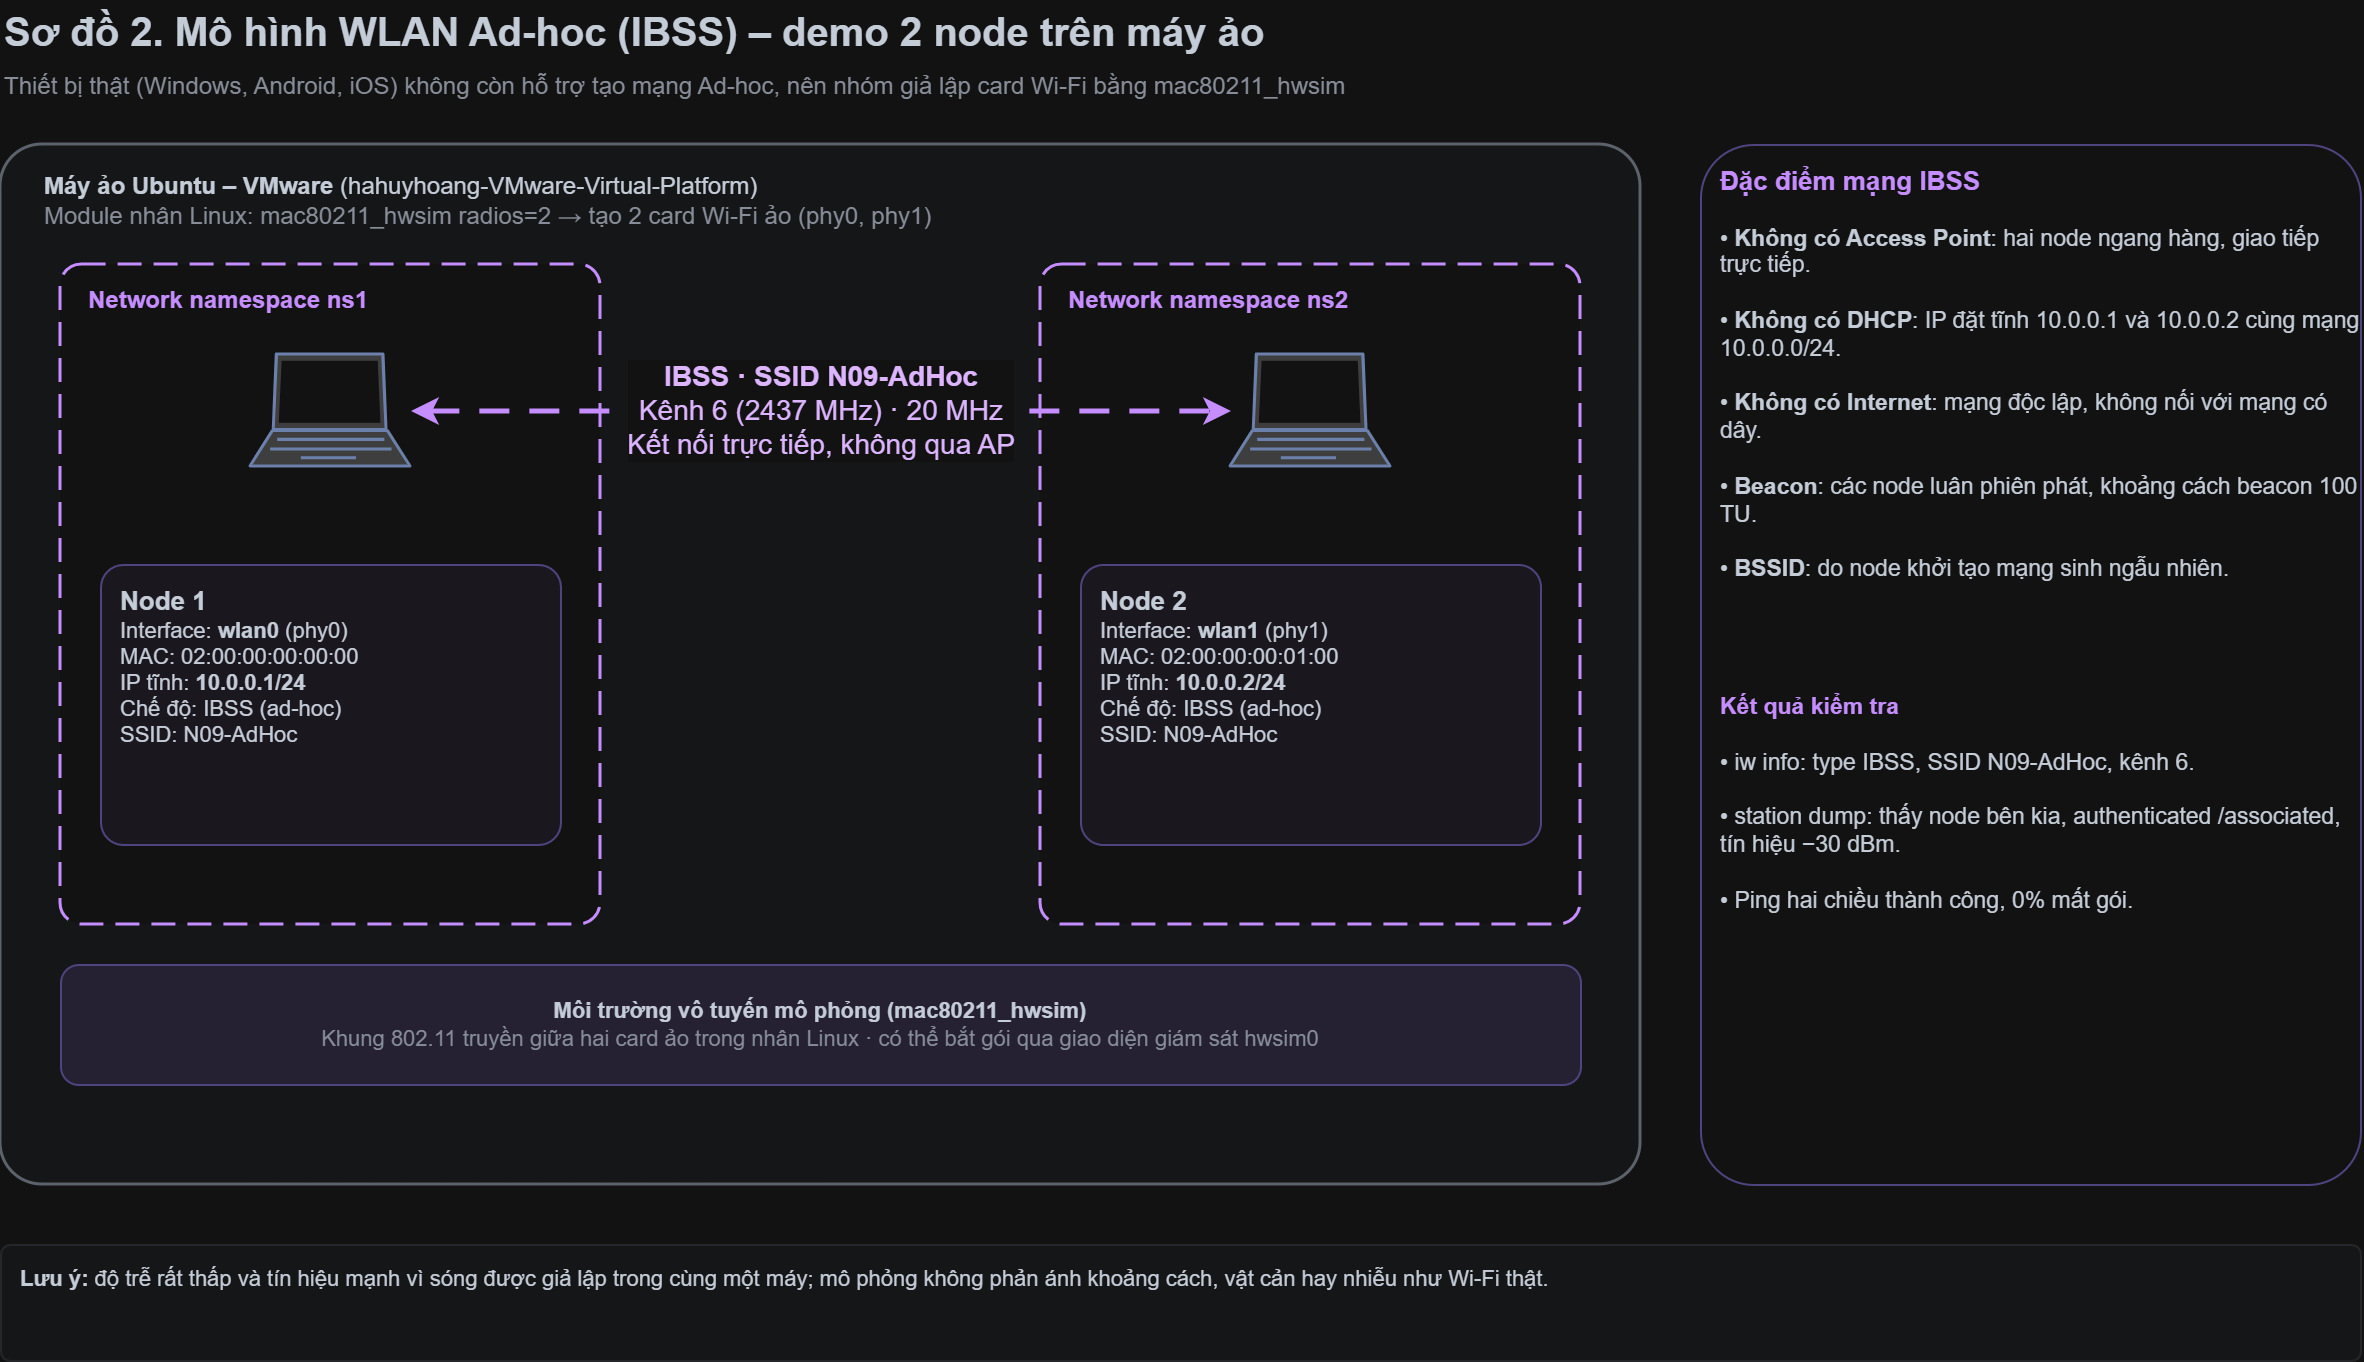
\includegraphics[width=\linewidth]{figures/N09_sodo2_adhoc.png}
  \caption[Sơ đồ mô hình Ad-hoc (IBSS) hai nút trên máy ảo]{Sơ đồ mô hình Ad-hoc (\ac{ibss}) hai nút trên máy ảo: hai card Wi-Fi ảo
  \texttt{phy0}, \texttt{phy1} được tách vào hai network namespace, cùng tham gia
  \ac{ibss} \texttt{N09-AdHoc} trên kênh~6 và giao tiếp trực tiếp, không qua
  \ac{ap}.}
  \label{fig:sodo-adhoc}
\end{figure}

\textbf{Định danh trong \ac{ibss}.} Ở mạng hạ tầng (\ac{bss}), \ac{bssid} là địa
chỉ MAC thật của \ac{ap}. Ở mạng Ad-hoc, vì không có \ac{ap}, nút đầu tiên khởi
tạo mạng sẽ tự sinh một địa chỉ MAC ảo ngẫu nhiên để làm \ac{bssid}; các nút
tham gia sau đó cùng dùng chung mã \ac{bssid} ảo này để nhận diện nhau.

\textbf{Duy trì mạng bằng beacon phân tán.} Trong \ac{bss}, \ac{ap} liên tục
phát khung beacon để thông báo mạng còn tồn tại. Trong \ac{ibss}, do các nút
bình đẳng, các nút tranh chấp cơ hội phát beacon tại mỗi thời điểm phát mục tiêu;
chu kỳ thường dùng là 100~TU. Nhờ đó không cần một nguồn
phát duy nhất mà mạng vẫn được duy trì.

\textbf{Tính cô lập.} \ac{ibss} là một ``hòn đảo'' độc lập: mặc định nó không
thể giao tiếp với hệ thống mạng có dây bên ngoài và không có kết nối Internet.
Đây là khác biệt bản chất so với mô hình hạ tầng, nơi \ac{ds} và bộ định tuyến
biên mở đường ra mạng ngoài.

\textbf{Giới hạn công nghệ.} Mạng Ad-hoc hoạt động ổn định nhất trên các chuẩn
Wi-Fi cũ là 802.11b, 802.11g và 802.11n ở băng tần 2,4~GHz. Về bảo mật, phần
lớn triển khai \ac{ibss} trên hệ điều hành phổ thông chỉ hỗ trợ mã hóa
\ac{wep} -- loại mã hóa đã bị chứng minh có thể bị phá trong vài phút -- hoặc
buộc phải để mạng mở không mật khẩu; do đó mô hình này không phù hợp cho dữ liệu
nhạy cảm. Ngoài ra, hiệu năng suy giảm rõ rệt khi số nút tăng, vì toàn bộ việc
điều phối kênh diễn ra phân tán và không có thiết bị nào quản lý tài nguyên vô
tuyến.

\textbf{Tiến hóa của mô hình.} Trên các thiết bị hằng ngày như điện thoại, máy
tính xách tay hay máy tính cá nhân, chế độ Ad-hoc đã được thay thế bằng
Wi-Fi Direct. Đối với các mạng như MANET, VANET hay FANET, đây là phiên bản
tiến hóa cao cấp nhất của mạng Ad-hoc: chúng vẫn thuần túy ngang hàng nhưng được
bổ sung các giao thức định tuyến (routing protocol) khá phức tạp ở tầng mạng
(lớp~3) để chuyển tiếp gói qua nhiều chặng, và vẫn đang được sử dụng trong những
lĩnh vực chuyên biệt như cứu hộ -- cứu nạn, giao thông thông minh hay thiết bị
bay không người lái.

\subsubsection{Mô hình hạ tầng do nhóm triển khai trên thiết bị thật}

Để phần lý thuyết gắn với thực nghiệm, nhóm triển khai mô hình hạ tầng trên một
bộ định tuyến thật là TP-Link Archer C20 v5 cài phần mềm OpenWrt, tên thiết bị
\texttt{N09-Router}, với địa chỉ quản trị \texttt{192.168.1.1}. Router có hai bộ
phát: bộ 2,4~GHz dùng chip MediaTek MT7628 theo chuẩn 802.11b/g/n và bộ 5~GHz
dùng chip MT7610E theo chuẩn 802.11ac.

Hình~\ref{fig:sodo-n09} là sơ đồ mạng mà nhóm đã dựng và đo được. Hai điểm đáng
chú ý về mặt lý thuyết:

\begin{itemize}[leftmargin=*]
  \item Mỗi bộ phát tạo một \ac{bss} riêng nên có \ac{bssid} riêng: bộ 2,4~GHz
    dùng \texttt{B0:95:75:9F:1C:A3} (kênh~6, 2,437~GHz, độ rộng 20~MHz), bộ
    5~GHz dùng \texttt{B0:95:75:9F:1C:A2} (kênh~36, 5,180~GHz, 802.11ac,
    WPA2-PSK/CCMP). Hai \ac{bssid} chỉ khác nhau một bit, phản ánh việc hai giao
    diện vô tuyến nằm trên cùng một thiết bị.
  \item Cả ba thiết bị di động trong mạng đều tự chọn liên kết vào \ac{bss}
    5~GHz, còn \ac{bss} 2,4~GHz không có trạm nào. Đây là minh chứng thực tế cho
    nhận định ở Mục~\ref{sec:arch}: việc chọn \ac{ap} và băng tần là do thiết bị
    đầu cuối quyết định, thường theo cường độ tín hiệu và băng thông hỗ trợ.
\end{itemize}

\begin{figure}[htbp]
  \centering
  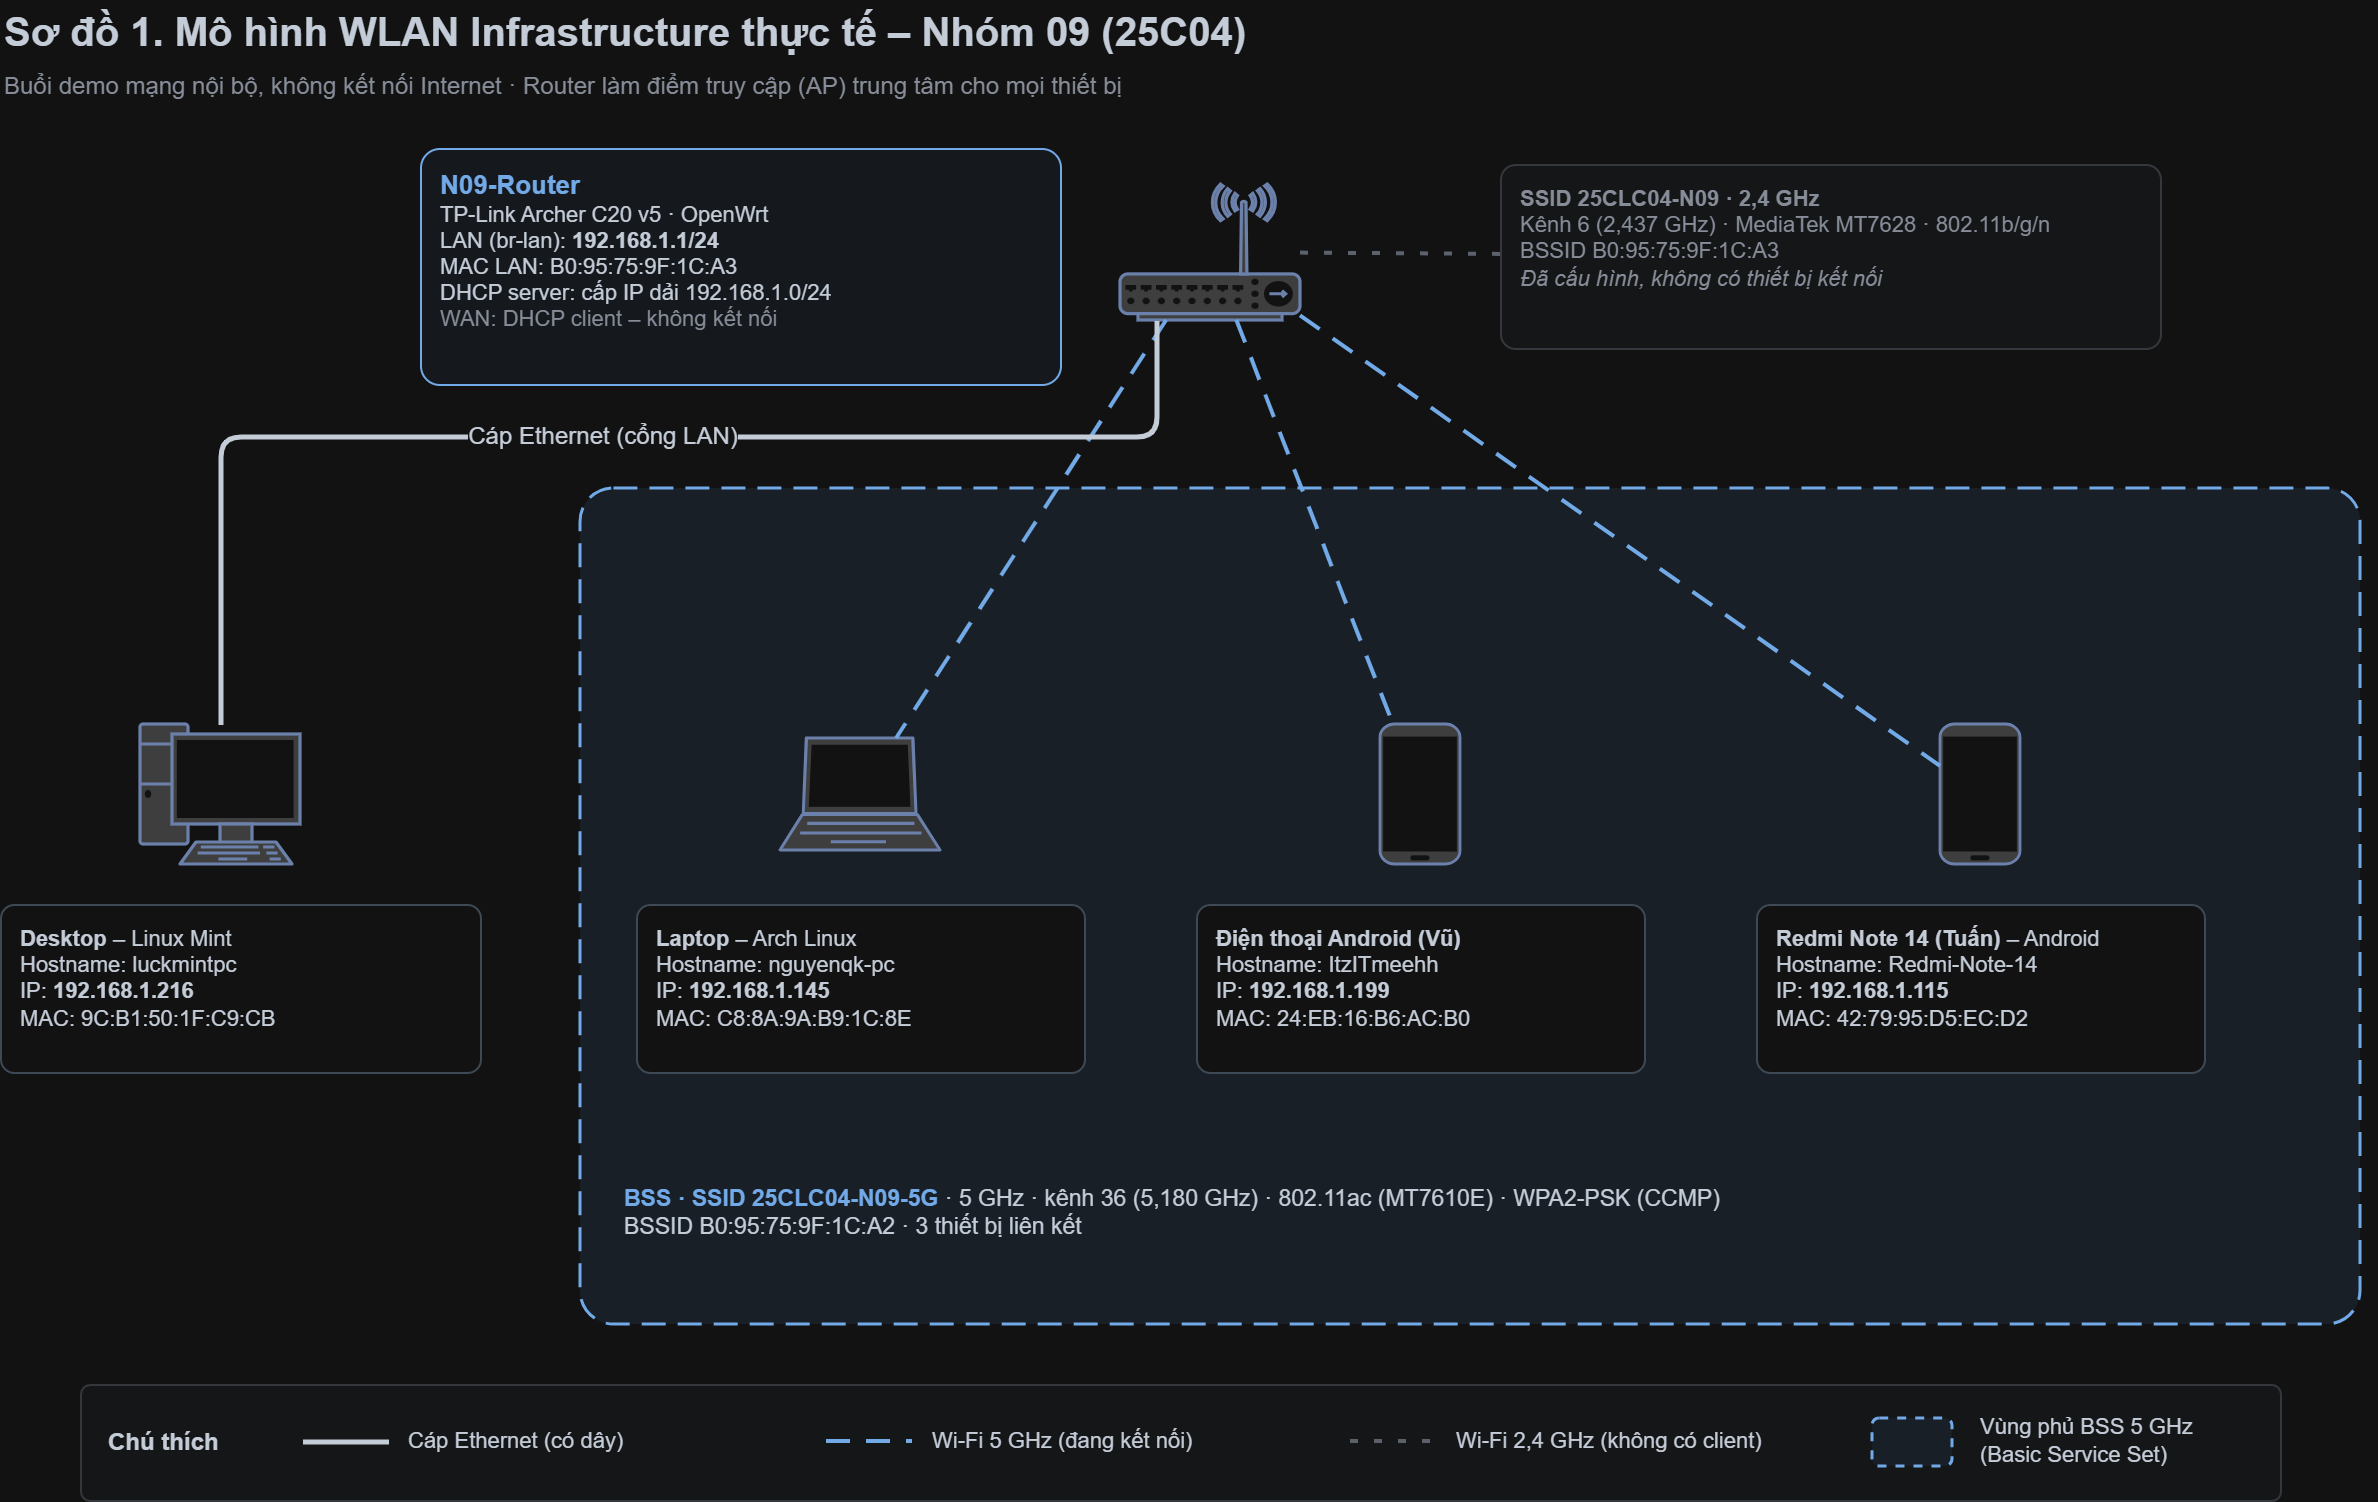
\includegraphics[width=\linewidth]{figures/N09_sodo1_infrastructure.png}
  \caption[Sơ đồ mô hình WLAN Infrastructure thực tế của nhóm]{Sơ đồ mô hình WLAN Infrastructure thực tế của nhóm: bộ định tuyến
  N09-Router (TP-Link Archer C20 v5, OpenWrt) làm \ac{ap} trung tâm, một máy bàn
  nối bằng cáp Ethernet vào cổng LAN và ba thiết bị di động liên kết vào
  \ac{bss} 5~GHz.}
  \label{fig:sodo-n09}
\end{figure}

\subsubsection{Đối chiếu chi tiết giữa hai mô hình}

Bảng~\ref{tab:infra-adhoc-detail} hệ thống hóa các khác biệt ở mức kiến trúc,
định danh, vận hành và bảo mật. Bảng này bổ sung cho bảng so sánh tổng quát
(Bảng~\ref{tab:infra-vs-adhoc}) bằng các tiêu chí cụ thể đã được kiểm chứng
trong quá trình thực nghiệm.

\begin{table}[htbp]
  \centering\footnotesize
  \caption{Đối chiếu chi tiết giữa mô hình hạ tầng (Infrastructure) và mô hình
  tùy biến (Ad-hoc / IBSS).}
  \label{tab:infra-adhoc-detail}
  \begin{tabularx}{\linewidth}{@{} L{0.75} L{1.15} L{1.1} @{}}
    \toprule
    \textbf{Tiêu chí} & \textbf{Mô hình hạ tầng (Infrastructure)} & \textbf{Mô hình tùy biến (Ad-hoc / \ac{ibss})} \\
    \midrule
    Thiết bị trung tâm & Bắt buộc có \ac{ap} hoặc bộ định tuyến không dây đảm
      nhiệm phát sóng và chuyển tiếp & Không có; các \ac{sta} hoàn toàn ngang
      hàng và tự chuyển tiếp cho nhau \\
    Đơn vị cấu thành & \ac{bss} (một \ac{ap}) mang \ac{bssid} riêng; nhiều
      \ac{bss} ghép thành \ac{ess} & \ac{ibss}: một nhóm nút độc lập, không có
      \ac{ap} \\
    Nguồn \ac{bssid} & Địa chỉ MAC vật lý của giao diện vô tuyến trên \ac{ap} &
      Địa chỉ MAC ảo sinh ngẫu nhiên bởi nút khởi tạo mạng, các nút khác dùng
      chung \\
    Phát beacon & \ac{ap} phát định kỳ, một nguồn phát duy nhất & Các nút phân
      tán cơ hội phát beacon; 100~TU là chu kỳ thường dùng \\
    Điều phối truy cập kênh & \ac{ap} giữ vai trò chủ; có thể hỗ trợ DCF hoặc
      PCF/HCCA & Phân tán hoàn toàn, chỉ hoạt động theo DCF (\ac{csmaca}) \\
    Cấp phát địa chỉ IP & Máy chủ DHCP tập trung trên \ac{ds} & Gán tĩnh thủ
      công, không có máy chủ DHCP \\
    Kết nối ra mạng ngoài & Có, qua \ac{ds} và bộ định tuyến biên & Mặc định
      không có; mạng bị cô lập với \ac{lan} có dây và Internet \\
    Mở rộng và chuyển vùng & Tốt; thêm \ac{ap} cùng \ac{ssid} là mở rộng
      \ac{ess}, hỗ trợ chuyển vùng & Kém; mọi nút phải trùng \ac{ssid} và trùng
      kênh, không có chuyển vùng; hiệu năng giảm khi số nút tăng \\
    Bảo mật & Đầy đủ; hỗ trợ WPA2/WPA3, 802.1X/\ac{radius} cho doanh nghiệp &
      Hạn chế; thực tế chỉ \ac{wep} hoặc mạng mở, không có WPA2/WPA3 \\
    Chuẩn và băng tần & Mọi thế hệ 802.11 và mọi băng tần được cấp phép & Ổn
      định nhất trên 802.11b/g/n, băng tần 2,4~GHz \\
    Hỗ trợ trên hệ điều hành phổ thông & Mặc định trên Windows, Android, iOS và
      macOS & Phụ thuộc hệ điều hành, driver và phần cứng; Linux thường cung cấp
      công cụ cấu hình IBSS đầy đủ hơn \\
    Ứng dụng thực tế & Gia đình, văn phòng, trường học, doanh nghiệp & Chia sẻ
      dữ liệu tạm thời, cứu nạn khẩn cấp, mạng cảm biến; nay chủ yếu được thay
      bằng Wi-Fi Direct \\
    \bottomrule
  \end{tabularx}
\end{table}

Từ đối chiếu trên có thể rút ra định hướng lựa chọn mô hình: hiệu năng, khả năng
mở rộng, kết nối Internet và bảo mật hiện đại là những lý do khiến mô hình hạ
tầng vẫn là mặc định cho mọi nhu cầu khai thác thực tế; mô hình Ad-hoc chỉ còn
giá trị ở những tình huống không thể dựng hạ tầng, hoặc trong các dạng tiến hóa
đa chặng phục vụ mục đích chuyên biệt. Chính vì giới hạn về bảo mật và khả năng
kết nối, phần Ad-hoc của báo cáo chỉ dùng chế độ \ac{ibss} để kiểm chứng nguyên
lý ngang hàng ở mức hai nút trên nền Linux
(Mục~\ref{sec:adhoc-config} và Mục~\ref{sec:experiment}), trong khi mọi nội dung
về bảo mật, cấp phát địa chỉ và kết nối Internet được kiểm chứng trên mô hình hạ
tầng với router thật.

\endgroup
